%Documento principal do latex para uso no TCC da Univás.
\documentclass[a4paper, 12pt, chapter=TITLE, oneside, english, brazil]{abntex2}
\usepackage{styles/CodeStyle}      %Formatação de códigos e listagens
\usepackage{styles/EventFlowStyle} %Estilo para o quadro de fluxo de eventos
\usepackage{styles/NuapaStyle}     %Estilo exigido pela Univás
 
%Início do documento
\begin{document}
  
\pretextual %Início dos Elementos Pré-Textuais


\makeatletter
\renewcommand{\imprimircapa}{%
\begin{capa}%
\begin{center}%
  {\ABNTEXchapterfont\large\MakeUppercase\imprimirautor}\\
  \vspace*{\fill}%
  \vspace*{\fill}%
  \vspace*{\fill}%
  {\ABNTEXchapterfont\bfseries\Large\MakeUppercase\imprimirtitulo}\\
  \vspace*{\fill}%
  {\color{white}%
\abntex@ifnotempty{\imprimirpreambulo}{%
  \hspace{.45\textwidth}
  \begin{minipage}{.5\textwidth}
    \SingleSpacing
    \imprimirpreambulo
  \vspace{.1\textwidth}\\%
  {\imprimirorientadorRotulo:~\imprimirorientador}
  \abntex@ifnotempty{\imprimircoorientador}{%
    \hspace{.45\textwidth}
    {\large\imprimircoorientadorRotulo~\imprimircoorientador}%
  }%
  \end{minipage}%
}%
\color{black}}%
  \vspace*{\fill}\\%
  {\ABNTEXchapterfont\large\bfseries\MakeUppercase\imprimirinstituicao}\\
  {\large\bfseries\MakeUppercase\imprimirlocal}\\
  {\large\bfseries\MakeUppercase\imprimirdata}
\end{center}
\end{capa}
}
\makeatother

\imprimircapa

% folha de rosto 
%\folhaderostoname{Folha de rosto}
%http://code.google.com/p/abntex2/wiki/ComoCustomizar

\makeatletter
\renewcommand{\folhaderostocontent}{
\begin{center}%
  {\ABNTEXchapterfont\large\MakeUppercase\imprimirautor}\\
  \vspace*{\fill}%
  \vspace*{\fill}%
  \vspace*{\fill}%
  {\ABNTEXchapterfont\bfseries\Large\MakeUppercase\imprimirtitulo}\\
  \vspace*{\fill}%
\abntex@ifnotempty{\imprimirpreambulo}{%
  \hspace{.45\textwidth}
  \begin{minipage}{.5\textwidth}
    \SingleSpacing
    \imprimirpreambulo
  \vspace{.1\textwidth}\\%
  %{\imprimirorientadorRotulo:~\imprimirorientador} <-- essa é a linha original, apenas retirei os : para o pré projeto(sem orientador)
  {\imprimirorientadorRotulo~\imprimirorientador}
  \abntex@ifnotempty{\imprimircoorientador}{%
    \hspace{.45\textwidth}
    {\large\imprimircoorientadorRotulo~:\imprimircoorientador}%
  }%
  \end{minipage}%
}%
  \vspace*{\fill}\\%
  {\ABNTEXchapterfont\large\bfseries\MakeUppercase\imprimirinstituicao}\\
  {\large\bfseries\MakeUppercase\imprimirlocal}\\
  {\large\bfseries\MakeUppercase\imprimirdata}
\end{center}
}%end of folhaderostocontent
\makeatother

\imprimirfolhaderosto*{}	
%\begin{fichacatalografica}
\begin{normalsize}
  \vspace*{\fill}
  % Posição vertical
%  \hrule
  % Linha horizontal
  \begin{center}
  \fbox{
    % Minipage Centralizado
    \begin{minipage}[c]{12.5cm} % Largura
      \vspace{0.7cm}%
      \hspace{0.8cm} \imprimirAutorCitacao ~\\%
      
      \hspace{0.8cm} \imprimirtitulo ~/ \imprimirAutorUm , \imprimirAutorDois ~-- \imprimirlocal: Univás, \imprimirdata. %
      
      \hspace{0.8cm} \pageref{LastPage} f. : il.~\\%
      
      \hspace{0.8cm} \imprimirtipotrabalho~--~\imprimirinstituicao , Univás, \imprimircurso. % 
      
      \hspace{0.8cm} \imprimirorientadorRotulo: ~\imprimirorientador ~\\%

      \hspace{0.8cm} 1. \imprimirPalavraChaveUm. 2. \imprimirPalavraChaveDois. 3. \imprimirPalavraChaveTres. ~ \\%
    \end{minipage}
    }
  \end{center}
\end{normalsize}
\end{fichacatalografica}
\newpage
%\setlength{\ABNTEXsignwidth}{10cm}

\begin{folhadeaprovacao}
  \begin{center}
    {\ABNTEXchapterfont\large\MakeUppercase\imprimirautor}
    \vspace*{\fill}
    \vspace*{\fill}
    \vspace*{\fill}
    \par
    {\ABNTEXchapterfont\bfseries\Large\MakeUppercase\imprimirtitulo}
    \vspace*{\fill}
  \end{center}
  Trabalho de conclusão de curso defendido e aprovado em \imprimirDataDaAprovacao ~pela banca examinadora constituída pelos professores:

  ~\newline
  \begin{flushleft}
  \assinatura*{\imprimirorientador \\ \imprimirorientadorRotulo }
  \assinatura*{\imprimirAvaliadorUm \\ \imprimirAvaliadorLabelUm }
  \assinatura*{\imprimirAvaliadorDois \\ \imprimirAvaliadorLabelDois}
  \end{flushleft}
  \vspace*{\fill}
  \vspace*{\fill}
\end{folhadeaprovacao}

%\begin{dedicatoria}
\vspace*{\fill}
\vspace*{\fill}
\vspace*{\fill}
\vspace*{\fill}
\vspace*{\fill}
\vspace*{\fill}
De \imprimirAutorUm.
\newline
%início da dedicatória do autor um
Dedico este trabalho \ldots 

\vspace*{\fill}
De \imprimirAutorDois.
\newline
%início da dedicatória do autor dois
Dedico este trabalho \ldots

\end{dedicatoria}

%\begin{agradecimentos}

De \imprimirAutorUm
\newline
%início do agradecimento do autor um
\par Agradeço \ldots

\vspace*{\fill}
De \imprimirAutorDois
\newline
%início do agradecimento do autor dois
\par Agradeço \ldots

\end{agradecimentos}





%\begin{epigrafe}
\vspace*{\fill}
\begin{flushright}
\textit{‘‘Complicar é simples, \\
simplificar que é complicado.\\
(Paulo Sérgio dos Santos)}
\end{flushright}
\end{epigrafe}

%% --- resumo em português ---

\begin{OnehalfSpacing} 

\noindent \imprimirAutorCitacaoMaiuscula. {\bfseries\imprimirtitulo}. {\imprimirdata}.  Monografia -- Curso de {\MakeUppercase\imprimircurso}, {\imprimirinstituicao}, {\imprimirlocal}, {\imprimirdata}.

\vspace{\onelineskip}
\vspace{\onelineskip}
\vspace{\onelineskip}
\vspace{\onelineskip}

\begin{resumo}
~\\
%início do texto do resumo
\noindent Este trabalho apresenta \ldots

%fim do texto do resumo
\vspace{\onelineskip}
\vspace*{\fill}
\noindent \textbf{Palavras-chave}: \imprimirPalavraChaveUm. \imprimirPalavraChaveDois. \imprimirPalavraChaveTres.
\vspace{\onelineskip}
\end{resumo}

\end{OnehalfSpacing}

%% --- resumo em inglês ---

\begin{OnehalfSpacing} 

\noindent \imprimirAutorCitacaoMaiuscula. {\bfseries\imprimirtitulo}. {\imprimirdata}.  Monografia -- Curso de {\MakeUppercase\imprimircurso}, {\imprimirinstituicao}, {\imprimirlocal}, {\imprimirdata}.

\vspace{\onelineskip}
\vspace{\onelineskip}
\vspace{\onelineskip}
\vspace{\onelineskip}

\begin{resumo}[Abstract]%
\begin{otherlanguage*}{english}%
\textit{
%início do texto do abstract
\noindent This work presents \ldots
%fim do texto do abstract
}

\vspace{\onelineskip}
\vspace*{\fill}
\noindent \textbf{Key words}: \imprimirKeyWordOne. \imprimirKeyWordTwo. \imprimirKeyWordThree.
\end{otherlanguage*}
\vspace{\onelineskip}
\end{resumo}

\end{OnehalfSpacing}

%%Lista de Figuras
\pdfbookmark[0]{\listfigurename}{lof}
\listoffigures*
\cleardoublepage

% Lista de Quadros
\pdfbookmark[0]{\listofquadrosname}{loq}
\listofquadros*
\cleardoublepage

%Lista de Tabelas
\pdfbookmark[0]{\listtablename}{lot}
\listoftables*
\cleardoublepage

%Lista de Códigos
\counterwithout{lstlisting}{chapter}
\pdfbookmark[0]{\lstlistingname}{lol}
%http://tex.stackexchange.com/questions/50031/how-to-remove-contents-line-from-table-of-contents
\begin{KeepFromToc}
\lstlistoflistings
\end{KeepFromToc}
\cleardoublepage

%%Lista de siglas
%ver http://marc.info/?l=tex-br&m=110566665520790 para colocar em ordem alfabética.

\begin{SingleSpace}

	\begin{siglas}
		\item[CPA] 		Comissão Própria de Avaliação
		\item[CSS] 		\textit{Cascading Style Sheets}
		\item[HTML] 	\textit{HyperText Markup Language}
		\item[SDK]  	\textit{Software Development Kit}
		\item[UNIVÁS]   Universidade do Vale do Sapucaí
	\end{siglas}

\end{SingleSpace}

%Sumário
%ver esse link para configuração de fonte: http://tex.stackexchange.com/questions/83377/how-to-change-chapter-font-style-in-the-middle-of-the-table-of-the-contents
\pdfbookmark[0]{\contentsname}{toc}
\begin{SingleSpace} 
\tableofcontents*
\end{SingleSpace}
\cleardoublepage


\textual %Início dos Elementos Textuais

%\chapter*{Introdução}
%\begin{center}
\vspace{1.2em}
\textbf{\large INTRODUÇÃO}

\vspace{2.9em}
%\end{center}
%\thispagestyle{empty} // Essa linha tira a numeração da página

\addcontentsline{toc}{chapter}{INTRODUÇÃO}
\stepcounter{chapter} %incrementa o número do capítulo

	\par No mundo em que vivemos, com o desenvolvimento tecnológico e os \textit{smartphones} em ascensão, as pessoas sempre olham seu dispositivo como recurso para resolver um problema ou como ele pode facilitar uma determinada tarefa, como uma transação bancária, uma pesquisa em um site de buscas ou simplesmente para acessar uma rede social. Esses dispositivos que estão na mão de praticamente todos os universitários, podem ser usados como grandes aliados de uma instituição de ensino. Hoje em dia, o desenvolvimento e a utilização de \textit{softwares} não se limita apenas aos \textit{desktops} como era a alguns anos atrás, cada vez mais os sistemas seguem atrelados aos dispositivos móveis, com toda a facilidade e mobilidade que eles nos proporcionam.
	
	\par O projeto consiste em criar uma aplicação que possibilite a universidade coletar opiniões dos alunos em relação à sua infraestrutura, professores, instalações, entre outros, algo que já é feito semestralmente através do portal do aluno, mas que pode ser aprimorado com o uso de um aplicativo destinado especialmente para esse objetivo. Uma pesquisa que seria realizada através do portal da universidade, que passa a ser feita por um aplicativo móvel, se torna ainda mais atrativa para quem possa vir a respondê-la. 

	\par A tecnologia que será usada no desenvolvimento do projeto, que é chamada de híbrida, permite que um único aplicativo possua suporte para mais de uma plataforma \textit{mobile}, como por exemplo o \textit{Android} e o \textit{iOS}, tudo isso a partir do \textit{framework} Ionic. De acordo com \citeonline{khanna2016getting}, aplicativos híbridos são semelhantes aos aplicativos nativos, eles são desenvolvidos com um único código base e utilizados em mais de uma plataforma, além possuírem comunicação com o \textit{hardware} e também serem instalados no dispositivo. Segundo \citeonline{ionicdesc} o Ionic é um poderoso SDK\footnote{\textit{Software Development Kit}} HTML5 que ajuda a construir aplicativos móveis usando tecnologias web como HTML\footnote{\textit{HyperText Markup Language}}, CSS\footnote{\textit{Cascading Style Sheets}} e Javascript, que são voltados principalmente para a interface gráfica do aplicativo.

\chapter{JUSTIFICATIVA}

	\par A escolha de falarmos sobre o Ionic e desenvolver um aplicativo usando seus conceitos, deve-se pela sua excelente forma de construir um App\footnote{Abreviação para a palavra \textit{Application}} \textit{mobile} multiplataforma, além das tecnologias usadas por ele que estão mais robustas e em constantes atualizações. A principal plataforma utilizada será o \textit{Android} devido à sua grande popularidade e por ser um dos Sistemas Operacionais mais usados mundialmente.
	
	\par A relevância do aplicativo frente à universidade é grande, pois facilitará na pesquisa que é feita pela CPA, a qual muitos alunos deixam de responder por falta da praticidade, que pode ser alcançada a partir de um aplicativo destinado especialmente para ela, com fácil utilização, intuitivo e que emite alertas aos usuários quando a pesquisa estiver disponível. Com a pesquisa atingindo seu público por mais de um meio, a quantidade de entrevistados aumenta, o que no final, garante ainda mais informações.
	
	\par O trabalho também auxiliará os alunos que se interessarem por aprender como funciona o desenvolvimento de um aplicativo híbrido, além de todas as tecnologias e \textit{frameworks} que estão envolvidos no processo, que são atuais e muito requisitadas no mercado de trabalho.
	

\chapter{OBJETIVOS}

	\par Descreveremos à seguir os objetivos pretendidos com base na presente pesquisa.

\section{Objetivo Geral}

	\par Desenvolver um aplicativo móvel multiplataforma a partir do \textit{framework} Ionic, que deve possibilitar aos alunos da UNIVÁS\footnote{Universidade do Vale do Sapucaí} responderem ao questionário semestral que é disponibilizado pela CPA\footnote{Comissão Própria de Avaliação} afim de coletar informações e opiniões referentes à universidade.

\section{Objetivos Específicos}

	\par Afim de atingir o objetivo geral da pesquisa, estão descritos a seguir os objetivos específicos.
	
	\begin{itemize}
		\item Levantamento de requisitos do sistema, bem como das tecnologias que serão usadas no desenvolvimento;
		\item Planejar o desenvolvimento do projeto a partir dos requisitos coletados;
		\item Desenvolver o aplicativo que permita aos alunos responderem o questionário da CPA.
	\end{itemize}
	\par Conforme esses objetivos, espera-se demonstrar de maneira simples e efetiva o funcionamento do Ionic e seu método de desenvolvimento híbrido, tirando o maior proveito possível com um software que auxiliará a pesquisa que é realizada pela CPA.


\chapter{QUADRO TEÓRICO}

	\par Para que se possa desenvolver uma aplicação são necessárias algumas tecnologias como linguagens de programação e \textit{frameworks}, falaremos no capítulo a seguir quais são eles e suas principais características.

\section{IONIC}
	\par Segundo \citeonline{ionicdesc} o \textit{framework} foi construído por benjsperry , adamdbradley e maxlynch em Drifty , uma empresa de \textit{software} independente e fabricantes de produtos reconhecidos como \textit{Codiqa} e \textit{Jetstrap}. O IONIC foi desenvolvido para possibilitar que aplicativos \textit{mobile} fossem desenvolvidos em sua base com HTML5.
	\par Atualmente o IONIC exige o uso de AngularJS, que será o próximo assunto, isso para fins de potencializar seu desenvolvimento. Além do AngularJS, o IONIC também usa \textit{Javascript} e CSS nativo.

	\subsection{CSS}
		\par Segundo \citeonline{silva2011css3} CSS é a abreviação para o termo em inglês \textit{Cascading Style Sheet}, traduzido para o
		português como folhas de estilo em cascata. A linguagem CSS tem por finalidade estilizar uma estrutura HTML para a apresentação de elementos. Como por exemplo: cores de fontes, tamanhos de texto, bordas arredondadas entre outros.
		\par De acordo com \citeonline{lie2005cascading} os primeiros vestígios de CSS são do ano de 1994, onde surgiu a necessidade de melhorar a aparência de uma página \textit{web} tendo como \textit{layout} um jornal, naquela época algumas coisas ainda eram impossíveis de se fazer, coisas que hoje em dia com o CSS3, encontramos facilmente em qualquer \textit{website}.
		\par Sendo assim, entendemos que o CSS faz todo o trabalho de estilizar e deixar páginas \textit{web} com uma interface amigável e melhor apresentada do que somente quando se tem HTML puro.
		
\section{AngularJS}
	\par AngularJS
	
\section{Cordova}
	\par Cordova

\section{PHP}
	\par PHP

\section{MySQL}
	\par MySQL

\section{HTML5}
	\par HTML5

\section{CSS}
	\par CSS
%\chapter{QUADRO METODOLÓGICO}
\label{cap:quadroMetodologico}
\section{Tipo de Pesquisa}
\section{Contexto de Pesquisa}
\section{Participantes}
\section{Instrumentos}
\section{Procedimentos}
\section{Cronograma}
\section{Orçamento}
%
\chapter{RESULTADOS} 

\par Aqui deve aparecer a descrição dos resultados obtidos.



%
\chapter{CONCLUSÃO} 

\par A conclusão deste trabalho é \ldots

\par Assim conclui-se que \ldots




\postextual %Início dos Elementos Pós-Textuais

%\citeoption{abnt-etal-cite=2}
\citeoption{ABNT-final}

%\bibliography{nuapatex-options, biblio}	 % insere as REFERENCIAS (arquivo biblio.bib)
\bibliography{biblio}			             % insere as REFERENCIAS (arquivo biblio.bib)
\addcontentsline{toc}{chapter}{REFERÊNCIAS} % adiciona o título no sumário

%\begin{apendicesenv}

%\apendicesname{APÊNDICES}
% Imprime uma página indicando o início dos apêndices
\partapendices*

\addcontentsline{toc}{chapter}{APÊNDICES}

\chapter*{Título do Apêndice I}
\label{apendice:1}

\par Aqui deve conter o texto do Apêndice~\ref{apendice:1}. Na Figura~\ref{fig:ap1:identificador} é ilustrada a primeira tela deste processo.
\captionsetup[figure]{list=no}
\begin{figure}[h!]
 \centerline{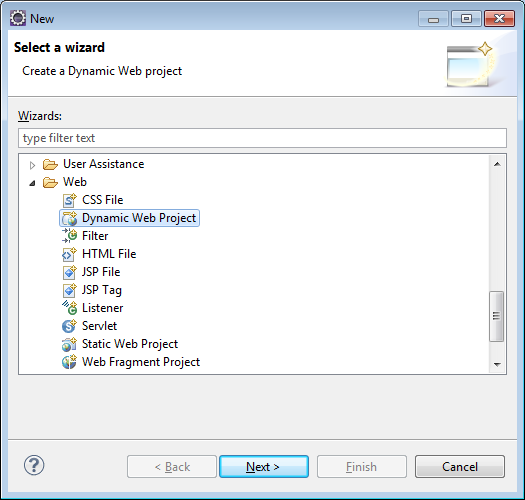
\includegraphics[scale=0.5]{./imagens/apendice_img1.png}}
 \caption[Outra imagem.]
           {Outra imagem. \textbf{Fonte:} Elaborado pelos autores}
  \label{fig:ap1:identificador}
\end{figure}

\par Após a seleção do tipo de projeto \ldots
\chapter*{Título do Apêndice 2}

\section*{Primeira seção do apêndice 2}

\par Neste apêndice é mostrado \ldots de acordo com a Figura~\ref{fig:ap2:identificador} é ilustrada a primeira tela deste processo.
\captionsetup[figure]{list=no}
\begin{figure}[h!]
 \centerline{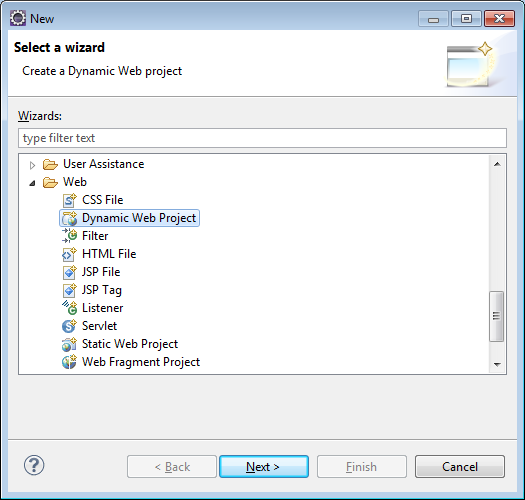
\includegraphics[scale=0.3]{./imagens/apendice_img1.png}}
 \caption[Outra imagem ainda.]
           {Outra imagem ainda. \textbf{Fonte:} Elaborado pelos autores}
  \label{fig:ap2:identificador}
\end{figure}

\section*{Segunda seção do apêndice 2}


\par Continuando \ldots na figura Figura~\ref{fig:xml_exemplo} é mostrado um exemplo de XML.

\begin{figure}[h!]
\begin{lstlisting}[style=custom_XML]
<project>
...
 <dependencies>
  ...
  <dependency>
   <groupId>org.neo4j</groupId>
   <artifactId>neo4j</artifactId>
   <version>1.9.4</version>
  </dependency>
  ...
 </dependencies>
 ...
</project>
\end{lstlisting}  
 \caption[Exemplo de código XML.]
           {Exemplo de código XML. \textbf{Fonte:} Elaborado pelos autores}
  \label{fig:xml_exemplo}
\end{figure}



\end{apendicesenv}
%%\anexoname{ANEXOS}
%\begin{anexosenv}
%\partanexos
%\chapter*{ANEXO I}

%\end{anexosenv}

\addcontentsline{toc}{chapter}{ANEXOS}

\chapter*{ANEXO I}



\printindex

\end{document}